% Figure 6 -- (a) Riemann sphere with one irregular and two regular punctures,
%             (b) its degeneration limit: two fundamentals and an AD point
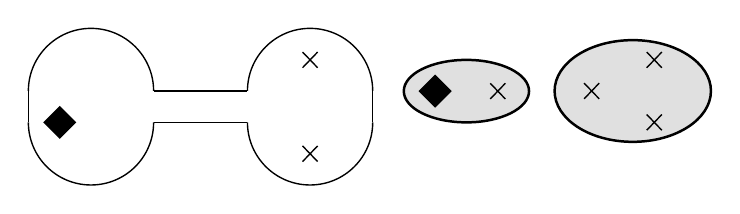
\begin{tikzpicture}[x=1pt,y=1pt,scale=1.05,transform shape,>=stealth,line width=0.5pt,
    bulb/.style={line width=0.5pt}, grey/.style={draw,fill=black!12,line width=0.9pt}]
  \def\cross#1#2{\draw (#1-2.6,#2-2.7) -- (#1+2.6,#2+2.7);\draw (#1-2.6,#2+2.7) -- (#1+2.6,#2-2.7);}
  % ---------- (a) dumbbell ----------
  \draw (51.6,35.0) arc[start angle=180,end angle=0,radius=21.55];
  \draw (51.6,24.2) arc[start angle=180,end angle=360,radius=21.55];
  \draw (51.6,24.2) -- (51.6,35.0);
  \draw (94.7,24.2) -- (127.0,24.2);
  \draw (94.7,35.0) -- (127.0,35.0);
  \draw (127.0,35.0) arc[start angle=180,end angle=0,radius=21.55];
  \draw (127.0,24.2) arc[start angle=180,end angle=360,radius=21.55];
  \draw (170.1,24.2) -- (170.1,35.0);
  % irregular puncture (filled diamond)
  \fill (56.7,24.2) -- (62.4,29.9) -- (68.1,24.2) -- (62.4,18.5) -- cycle;
  % two regular punctures
  \cross{148.55}{13.4}
  \cross{148.55}{45.7}
  % ---------- (b) the two pieces ----------
  \draw[grey] (202.35,34.95) ellipse[x radius=21.55pt,y radius=10.75pt];
  \fill (185.9,34.95) -- (191.6,40.65) -- (197.3,34.95) -- (191.6,29.25) -- cycle;
  \cross{213.15}{34.95}
  \draw[grey] (259.6,35.0) ellipse[x radius=26.9pt,y radius=17.5pt];
  \cross{245.45}{35.0}
  \cross{267}{24.2}
  \cross{267}{45.7}
\end{tikzpicture}
